\section*{Общая характеристика работы}

\subsection*{Актуальность темы}

Задачи деформаций и разрушения сложных конструкций представляют особый интерес для многих областей техники. Механика разрушения ставит множество как академических проблем, касающихся механизмов разрушения материалов различных типов, так и инженерных задач, связанных с требованиями обеспечить необходимые уровни надежности различных изделий.

Решение задач прочности конструкций сложной формы и реологии при непростых условиях нагружения трудно представить без применения компьютерного моделирования и эффективных численных методов. На сегодняшний день наиболее широкое распространение для данного класса задач получил метод конечных элементов (МКЭ). Основные параметры, используемые для описания условий разрушения в расчётах прочности методом конечных элементов, -- коэффициент интенсивности напряжений, J-интеграл, раскрытие в вершине трещины. Применение МКЭ и данных критериев позволяет эффективно решать статические задачи прочности.

Однако, для определения деформаций и повреждений в сложных конструкциях при динамической нагрузке требуется разработка методов, учитывающих волновые процессы при соударении. Особенно актуальна эта задача для многослойных и неоднородных материалов, в которых итоговая сложная картина повреждений формируется в результате множественных взаимодействий упругих и пластических волн как с внешними, так и с внутренними контактными границами. Ярким примером таких материалов являются современные композиты.

На сегодняшний день композиционные материалы активно внедряются во многих областях техники. Их использование открывает новые перспективы в авиастроении, космической отрасли, машиностроении и других отраслях благодаря сочетанию лёгкости и высокой прочности. В том числе активно рассматривается возможность применения композиционных материалов в ответственных силовых конструкциях оперения, крыла и фюзеляжа самолёта, что позволит значительно снизить массу конструкции. Благодаря этому станет возможной реализация новых конструктивно-силовых схем и компоновок летательных аппаратов и улучшения их характеристик.

В связи с этим важными задачами являются как разработка новых усовершенствованных 
композиционных материалов, так и создание методик и норм проверки их прочностных характеристик 
и надёжности в эксплуатации. Существующие методы проверки монолитных изделий из металлов и сплавов оказываются неэффективны для композитов в силу их сложной внутренней структуры.

Данная работа непосредственно связана с одной из актуальных прикладных задач 
прочностных испытаний композиционных материалов -- изучение поведения материала при 
динамической нагрузке. В силу анизотропности свойств композиционные материалы после
действия нагрузки могут заметно терять прочность даже при отсутствии видимых поврежедний.
Это обусловлено появлением микротрещин, которые впоследствии, объединяясь,
превращаются в макротрещины. Так, возникающее после нагрузки расслоение
материала может быть визуально не заметно, хотя делает образец непригодным к
дальнейшему использованию.

Разрушение композиционных материалов может происходить как в объеме (при сжатии, растяжении, 
сдвиге), так и на контактных границах между матрицей и наполнителем. В зависимости от типа 
нагрузки разрушение может носить деформационный или волновой характер. 
Динамическое воздействие вызывает распространение упругих волн в образце. В случае 
композиционного материала множественные переотражения волн от внутренних контактных 
границ между слоями создают сложную волновую картину. Интерференция прямых, отражённых 
и преломлённых волн формирует итоговые области максимальных нагрузок в конструкции.

В связи с этим для моделирования необходимо использовать численный метод решения системы 
уравнений механики деформируемого твёрдого тела, позволяющий получить полную волновую 
картину с высоким временным и пространственным разрешением с учётом влияния контактных 
границ. Указанными свойствами обладает сеточно-характеристический численный метод, 
применяемый в данной работе.

Для моделирования реальных инженерных конструкций необходимо разработать и реализовать численные методы, позволяющие выполнять расчёты в областях сложной геометрии. Для решения задач большой размерности требуется параллельная реализация используемых численных методов, обладающая высокой эффективностью при использовании на современных высокопроизводительных вычислительных комплексах.

\subsection*{Цели работы}

\begin{enumerate}
\item Разработка математических моделей для задачи низкоскоростного удара по инженерной конструкции, выполненной из композиционных материалов.
\item Разработка сеточно-характеристического метода, позволяющего выполнять расчёты на сетке из тетраэдров с шагом $\tau > h / \lambda$ (здесь $\tau$ -- шаг по времени, $h$ -- минимальное расстояние от узла сетки до соседних узлов, $\lambda$ -- максимальное по модулю собственное число упределяющей системы уравнений).
\item Разработка параллельной версии сеточно-характеристического метода с явным выделением контактных границ, обеспечивающей высокую эффективность при использовании на современных высокопроизводительных вычислительных комплексах.
\item Создание комплекса программ для решения прикладных задач. Интеграция комплекса с существующими сторонними программами задания геометрии объектов и визуализации результатов расчётов, являющимися стандартом де-факто среди инженеров-практиков.
\item Исследование волновых процессов в средах сложной структуры, численное решение задач об объёмных волнах, поверхностных волнах, волнах на контактной границе.
\item Исследование волновых процессов в элементе композитной обшивки и силового кессона крыла самолёта, приводящих к повреждениям конструкции при низкоскоростном ударе.
\end{enumerate}

\subsection*{Научная новизна}

\begin{enumerate}

\item Разработан метод численного моделирования на неструктурированной сетке действия низкоскоростного удара на конструкцию сложной формы в трёхмерной постановке. Разработанный метод позволяет проводить моделирование волновых процессов в конструкции при динамическом внешнем воздействии с учетом взаимодействия волновых фронтов, влияния внешних и внутренних границ, различия реологических свойств слоёв. Особенностью метода является возможность выполнять расчёты с шагом $\tau > h / \lambda$ в трёхмерной постановке. Разработанный метод исследован на аппроксимацию и устойчивость. Проведено тестирование реализации метода.

\item Разработанный сеточно-характеристический метод реализован в виде параллельного вычислительного комплекса, позволяющего выполнять моделирование как на стандартном оборудовании, так и на современных высокопроизводительных вычислительных комплексах.

\item Выполнено исследование волновых процессов в многослойных средах различной структуры, моделирующих панель из полимерного композиционного материала. Исследование включает в себя как аналитическое, так и численное изучение процессов, протекающих в многослойной среде при динамическом нагружении. Получены поля скоростей и напряжений, области потенциальных разрушений различных типов, обусловленные распространением и взаимодействием волновых фронтов в материале.

\item Выполнено численное моделирование натурного эксперимента по динамическому нагружению элемента композитной обшивки и силового кессона крыла самолёта. Проведены расчеты для двух постановок эксперимента -- удар по отдельному элементу обшивки и удар по элементу обшивки со стрингером. Для задачи со стрингером рассмотрены постановки с центральным и нецентральным ударом. Проведен анализ причин разрушения композиционных авиационных материалов. Для всех постановок получены области концентрации напряжений, вызванные волновыми процессами в ходе соударения. Определены зоны потенциальных повреждений конструкции, обусловленные разными механизмами разрушения материала. Для элемента обшивки без стрингера размер разрушенной области составляет 50-60 мм, для элемента обшивки со стрингером 25-30 мм при центральном ударе и 20-25 мм при нецентральном ударе.

\item Получено, что наличие стрингера существенно разгружает элемент обшивки при динамическом воздействии и уменьшает размер потенциально повреждённых областей. Данный результат важен, так как при действии статической нагрузки наличие стрингера напротив вызывает концентрацию напряжений и приводит к разрушению при меньшей силе воздействия.

\item Разработанный численный метод применен для решения ряда задач биомеханики. Получены области потенциальных повреждений тканей организма человека в задачах о черепно-мозговой травме, о динамическом нагружении коленного сустава и об ударе по торсу в защитной конструкции.

\end{enumerate}

\subsection*{Практическая ценность}

Результаты численного моделирования действия низкоскоростного удара на конструкцию из полимерного композиционного материала могут быть использованы для экспериментальной проверки предложенных математических моделей и численного метода. В работе сформулированы критерии для сравнения численного и натурного эксперимента, учитывающие механические свойства распространённых полимерных матриц.

После экспериментальной верификации разработанные модели и методы могут быть использованы при создании методик и норм проверки прочностных характеристик композиционных материалов.

Полученные результаты по взаимодействию упругой волны с разрушенной областью конструкции могут быть использованы при разработке методов неразрушающего контроля состояния изделий из композиционных материалов.

Кроме того, разработанный параллельный программный комплекс может быть использован для моделирования динамического воздействия на комплексные силовые конструкции из композиционных материалов в тех случаях, когда проведение натурных испытаний затруднительно.

Полученные результаты в части задач биомеханики могут быть использованы при разработке защитного снаряжения различных видов.

Работа поддержана рядом государственных и коммерческих грантов.

\begin{enumerate}

\item Федеральное государственное унитарное предприятие <<Российский Федеральный Ядерный Центр -- Всероссийский научно"=исследовательский институт экспериментальной физики (ФГУП <<РФЯЦ-ВНИИЭФ>>)>>. НИР5. <<Разработка физико-математических моделей, алгоритмов и эффективных методов решения задач механики сплошных сред на супер-ЭВМ>>;

\item Грант РФФИ 10-01-92654-ИНД\_а <<Математическое моделирование сложных задач на высокопроизволительных вычислительных системах>>, 2010--2011гг.

\item Грант РФФИ 11-01-00723-а <<Разработка численных методов моделирования динамических задач биомеханики на современных высокопроизводительных вычислительных системах>>, 2011--2013гг.

\item Грант РФФИ 10-01-00572-а <<Разработка алгоритмического обеспечения и вычислительных методов для численного решения задач динамики деформируемых сред на многопроцессорных ЭВМ нового поколения>>, 2010--2012гг.

\end{enumerate}

\subsection*{Публикации}

Научные результаты диссертации опубликованы в 12 работах, из которых две [8, 9] -- в изданиях, рекомендованных ВАК для публикации основных результатов диссертации.

\subsection*{Апробация}

Результаты работы были доложены, обсуждены и получили одобрение специалистов на следующих научных конференциях:

\begin{enumerate}
\item Научные конференции Московского физико-технического института <<Проблемы фундаментальных и прикладных, естественных и технических наук в современном информационном обществе>> (МФТИ, Долгопрудный, 2006--2011);
\item I международная конференция <<Математические модели и численные методы в биоматематике>> (Институт вычислительной математики РАН, Москва, 2010);
\item II международная конференция <<Математические модели и численные методы в биоматематике>> (Институт вычислительной математики РАН, Москва, 2011);
\item Расширенный семинар <<Вычислительная физика: алгоритмы, методы и результаты>> (представительство Института космических исследований РАН, Таруса, 2011);
\item The 8th Congress of the International Society for Analysis, its Applications, and Computation (ISAAC 2011) (Российский университет дружбы народов, Москва, 2011);
\item Российско-индийский семинар <<Новые достижения математического моделирования>> (Институт автоматизации проектирования РАН, Москва, 2011);
\item Международный авиационно-космический семинар им. С.М. Белоцерковского (Центральный аэрогидродинамический институт имени профессора Н.Е. Жуковского, Москва, 2012).
\end{enumerate}

Результаты работы были доложены, обсуждены и получили одобрение специалистов на научных семинарах в следующих организациях:
\begin{enumerate}
\item Центральный аэрогидродинамический институт имени профессора Н.Е. Жуковского (Москва--Жуковский, 2011, 2012);
\item Научно-исследовательский институт природных газов и газовых технологий – Газпром ВНИИГАЗ (Москва, 2011);
\item Институт вычислительной математики РАН (Москва, 2010, 2011);
\item Институт автоматизации проектирования РАН (Москва, 2011).
\end{enumerate}

\subsection*{Структура и объем диссертации}

Диссертация состоит из введения, пяти глав, заключения и списка использованных источников. Общий объем диссертации составляет 194 страницы. Список использованных источников содержит ссылки на 79 публикаций.

\subsection*{Содержание работы}

%В диссертационной работе рассматриваются задачи механики деформируемого твердого тела, связанные с деформациями и повреждениями сложных конструкций при действии динамической внешней нагрузки. Для решения указанных задач конструируется сеточно-характеристический метод на неструктурированной сетке для случая трех пространственных переменных и низкого качества расчетной сетки. Метод реализуется в виде параллельного программного комплекса. С применением разработанного метода исследуются волновые процессы в многослойных средах, рассчитывается задача о низкоскоростном ударе по элементу композитной обшивки и силового кессона крыла самолёта, выполняются тестовые расчета ряда задач биомеханики.


\subsubsection*{Введение}

Во введении обсуждается актуальность темы диссертации, описываются основные цели работы, формулируется новизна работы и ее практическая ценность, указываются положения, выносимые на защиту.

\subsubsection*{Глава 1}

В первой главе рассматриваются математические модели деформируемого твердого тела. Используется система динамических уравнений в виде
\begin{align}
\label{initial_equations}
\rho\dot{v}_i &= \nabla_j\sigma_{ij}+f_i & \textrm{(уравнения движения)}\nonumber\\
\sigma_{ij} &= q_{ijkl}\dot{\varepsilon}_{kl}+F_{ij} & \textrm{(реологические
соотношения).}
\end{align}

Здесь $\rho$ – плотность среды, $v_i$ – компоненты скорости смещения,
$\sigma_{ij}$, $\varepsilon_{ij}$ -- компоненты тензоров напряжений и деформаций,
$\nabla_j$ – ковариантная производная по $j$-й координате, $f_i$ – массовые
силы, действующие на единицу объёма, $F_{ij}$ -- правая часть, используемая, например, для описания диссипации в моделях с учётом вязкости.

Вид компонент тензора 4-го порядка $q_{ijkl}$ и правой части $F_{ij}$ определяется реологией среды.

В работе используются различные модели линейно"=упругого тела, упруго"=пластического тела (модель Прандтля"=Рейсса), вязко"=упругого тела (модель Максвелла и модель Работнова), вязко"=упруго"=пластического тела (модель Кукуджанова). Для всех математических моделей формулируется матричная форма записи системы определяющих уравнений в частных производных в виде
\begin{equation}
\label{matrix_equation}
\frac{\partial\vec{u}}{\partial{t}}+\mathbf{A}_x\frac{\partial\vec{u}}{\partial{x}}+
\mathbf{A}_y\frac{\partial\vec{u}}{\partial{y}}+
\mathbf{A}_z\frac{\partial\vec{u}}{\partial{z}}=\vec{f}.
\end{equation}
Здесь $\vec{f}$ -- вектор правых частей, размерность которого равна размерности исходной системы, а выражения для компонентов зависят от реологии среды. Точный вид матриц $\mathbf{A}_x$, $\mathbf{A}_y$, $\mathbf{A}_z$ и вектора $\vec{f}$ зависит от реологии среды, аналитические выражения для всех компонентов матриц и вектора приведены в тексте диссертации.

В первой главе исследуются свойства матрицы общего вида $A_q$, возникающей при смене базиса в ходе решения уравнения \eqref{matrix_equation}. Смена базиса является частой операцией при практической реализации численного метода. Получено, что собственные числа $\lambda_i$ матрицы $A_q$ имеют вид:
\begin{align}
\left( \begin{array}{cccccccccccc}
\lambda_1 \\
\lambda_2 \\
\lambda_3 
\end{array} \right) = 
\frac 1 \rho (q_x^2 + q_y^2 + q_z^2)
\left( \begin{array}{cccccccccccc}
(\lambda+2\mu) \\
\mu \\
\mu  
\end{array} \right),
\end{align} 
где $\lambda$ и $\mu$ -- параметры Ламе, $q_i$ -- производные базисных векторов нового базиса по старому базису.

Таким образом, если оба базиса ортонормированные, собственные числа не меняются. В случае же перехода в неортонормированный базис собственные числа могут меняться в широком диапазоне.

От $\lambda_i$ напрямую зависит, какие точки на предыдущем шаге по времени будут нужны для реконструкции решения на новом временном слое. Чем больше значения $\lambda_i$, тем больше угол наклона характеристики. При увеличении $\lambda_i$ следует ожидать уменьшения допустимого шага по времени (при использовании курантовского ограничения на шаг), либо (при попытке сохранить шаг по времени неизменным) появление непредусмотренных характеристик, выводящих за пределы расчетной области. Способы построения численного метода, позволяющего решить эти проблемы, рассмотрены в главе 2 диссертации.

Также в первой главе рассматриваются различные модели разрушения, реализованные в дальнейшем в вычислительном комплексе, и обсуждаются подходы к моделированию композиционных материалов.

\subsubsection*{Глава 2}

Вторая глава посвящена сеточно-характеристическому численному методу. Рассматриваются гиперболические свойства определяющей системы уравнений и конструирование метода на их основе.

Обсуждаются численные методы первого и второго порядка точности на структурированных и неструктурированных сетках, применение гибридизации для повышения качества численного решения. Дается схема расчета внутренних, граничных и контактных узлов сетки. Приводится описание алгоритма перехода от одномерной задачи к многомерной с использованием расщепления разных порядков точности. Также рассматривается алгоритм выделения контактных границ и зон контакта тел в трехмерном случае при взаимном движении тел и деформациях сетки.

Отдельно во второй главе описывается конструирование метода для работы на неструктурированной сетке, позволяющего выполнять расчет с большим шагом по времени.

Одной из принципиальных проблем, с которыми сталкивается метод характеристик на сетках из тетраэдров при попытке расчета им реальных задач, является качество сеток, создаваемых стандартными генераторами сеток. Формально сеточно-характеристический метод может использоваться на любой сетке из тетраэдров. Однако, для сеток из тетраэдров имеет место ограничение на шаг по времени, аналогичное курантовскому шагу для равномерной прямоугольной сетки. Так для каждого узла сетки:

\begin{equation}
\tau \le \frac{\min(h)}{\max(|\lambda|)},
\end{equation}

где $\min(h)$ -- минимальная высота тетраэдра, в которые входит данный узел, $\max(|\lambda|)$ -- максимальное по модулю собственное число матрицы $\mathbf A$ для данного узла.

С практической точки зрения крайне нежелательна ситуация, когда $\tau$ оказывается малым для отдельных узлов сетки, так как это накладывает ограничения на шаг по времени для всей сетки. В связи с этим логично ввести критерий качества сетки в следующем виде:
\begin{equation}
q = \frac{\min(h)}{h_*},
\end{equation}
где $h_*$ -- заданная желаемая мелкость сетки, а $\min(h)$ -- минимальная высота в сетке, фактически выданной генератором.

Для идеальной сетки $q = 1$. Как показано в диссертации, на практике даже для простейшей геометрии $q$ находится в диапазоне $0.00065 \le q \le 0.126$, причем проблема носит систематический характер. Это приводит к неоправданному падению шага по времени на 1-3 порядка и, соответственно, к необоснованному росту требуемого объема вычислений.

В работе предлагается подход к модификации численного метода для обеспечения эффективной работы на такой сетке. Данный подход может применяться не только для решения проблемы малого шага по времени из-за топологии изначальной сетки, но и в случае деградации шага по времени из-за вырождения сетки в зоне больших деформаций.

Особенностью предлагаемого метода является тот факт, что необходимые точки на предыдущем временном слое, по которым выполняется реконструкция значений на следующем шаге по времени, определяются в ходе вычислений отдельно для каждой рассчитываемой точки, исходя из локальных свойств решения в ней.

Предположим, что из тех или иных соображений был выбран шаг по времени $\tau$, такой что характеристика из точки $u_m^n$ не попадает в отрезок $(u_{m-1}^n; u_{m+1}^n)$.

В этом случае найдем тот отрезок $(u_{m-k-1}^n; u_{m-k}^n)$, в котором выпущенная характеристика пересекает временной слой $n$. Точку пересечения обозначим $x^*$. Также введем обозначения:
\begin{align}
x_{m-k} - x_{m-k-1} &= h_k,\nonumber\\
x_m - x^* = \lambda \tau &= l_0,\nonumber\\
x_m - x_{m-k} &= l_k.
\end{align}

Нормируя $l_k$ и $l_0$ на $h_k$ получаем:
\begin{align}
q_0 &= l_0 / h_k = \lambda \tau / h_k = \sigma,\nonumber\\
q_k &= l_k / h_k,
\end{align}
где $\sigma$ -- аналог классического числа Куранта для равномерной сетки.

Для одномерного уравнения переноса и линейной интерполяции значения в точке $u_*^n$ по точкам  $u_{m-k-1}^n$ и $u_{m-k}^n$ получаем для значения на новом временном слое $u_m^{n+1}$ следующее выражение:
\begin{align}
\label{newmethod_1d_scheme}
u_m^{n+1} = u_*^n = (q_k + 1 - q_0) u_{m-k}^n + (q_0 - q_k) u_{m-k-1}^n.
\end{align}

Исследование метода на аппроксимацию и устойчивость, а также результаты тестирования метода на модельных задачах приведены в диссертации. Получено, что схема имеет первый порядок по времени и по пространству, является монотонной, устойчива при выполнении условия
\begin{align}
k \le \sigma \le k+1.
\end{align}

Тестирование на задаче распада разрыва показывает, что, несмотря на формальный первый порядок по пространству, разработанный метод лучше воспроизводит точное решение, чем схема <<явный уголок>>, также имеющая первый порядок аппроксимации.

На основании исследованного метода для одномерного уравнения и схемы расщепления по пространственным переменным в работе предлагается обобщение метода на многомерный случай (см. рис. \ref{pic:method_3d}).

\begin{figure}[ht]
\begin{subfigure}[b]{0.5\textwidth}
\centering
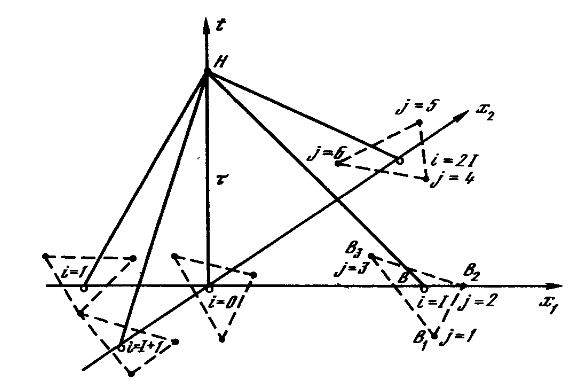
\includegraphics[width=\textwidth]{png/characteristics-2d-triangles-inner.png}
\caption{Расчет внутреннего узла.}
\end{subfigure}
\begin{subfigure}[b]{0.5\textwidth}
\centering
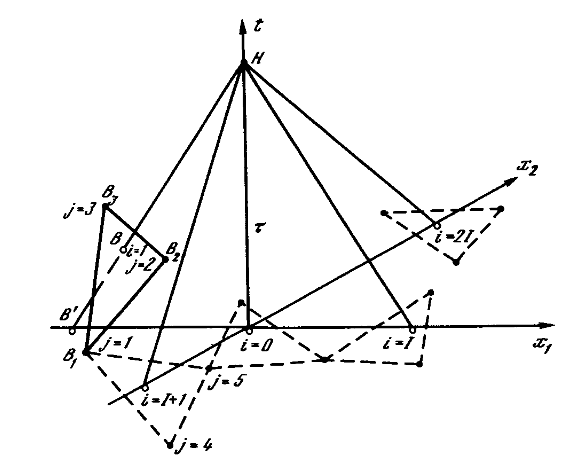
\includegraphics[width=\textwidth]{png/characteristics-2d-triangles-semi-border.png}
\caption{Расчет узла, близкого к границе.}
\end{subfigure}
\caption{К конструированию многомерной схемы.}
\label{pic:method_3d}
\end{figure}

В заключительной части второй главы рассматривается алгоритм параллельной версии разработанного сеточно-характеристического численного метода и архитектура параллельного программного комплекса. Отличительной особенностью реализованного параллельного алгоритма является возможность выполнять расчеты как методом сквозного счета неоднородностей, так и с явным выделением контактных границ. Для этого разработана и реализована параллельная версия детектора столкновений, обеспечивающая поиск зон контакта тел при их взаимном движении и деформациях. Результаты тестирования производительности параллельной версии приведены на рисунке \ref{pic:gcm_boost}.
\begin{figure}[htp]
\centering
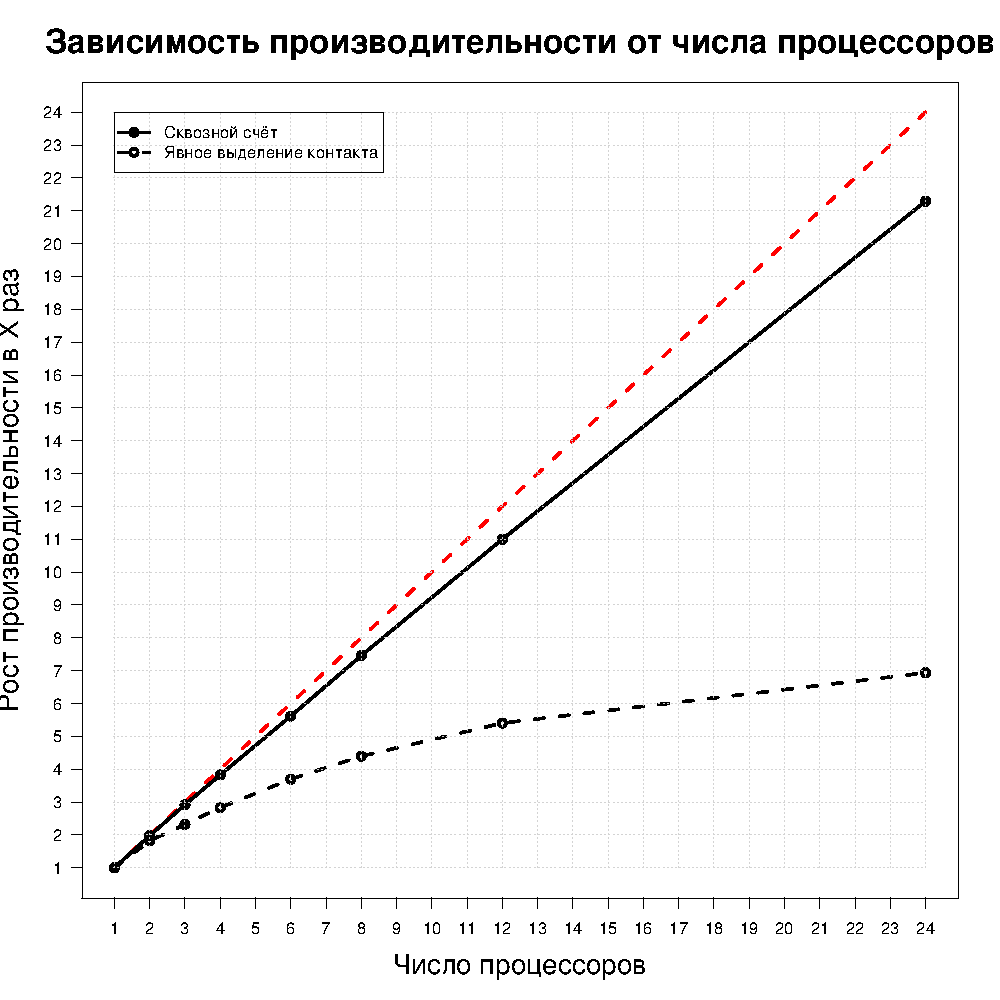
\includegraphics[width=0.5\textwidth]{eps/gcm3d-boost.eps}
\caption{Зависимость производительности от количества вычислительных узлов.}
\label{pic:gcm_boost}
\end{figure}

%\clearpage
%\newpage

\subsubsection*{Глава 3}

В третьей главе приведено исследование волновых процессов в средах сложной структуры. Получены как аналитические, так и численные решения. Получены решения для объемных волн (S-волна, P-волна), поверхностных волн (волны Рэлея и Лэмба, отражение сферической волны от свободной границы), волн на контактной границе (преломление на границе, волны Стоунли и Лява).

Для примера на рис. \ref{pic:stounly_wave} изображены результаты расчёта волн Стоунли при ударе по пятислойной преграде. Аналогичные результаты расчетов волн других типов приведены в тексте диссертации.

\begin{figure}[ht]
\begin{subfigure}[b]{0.5\textwidth}
\centering
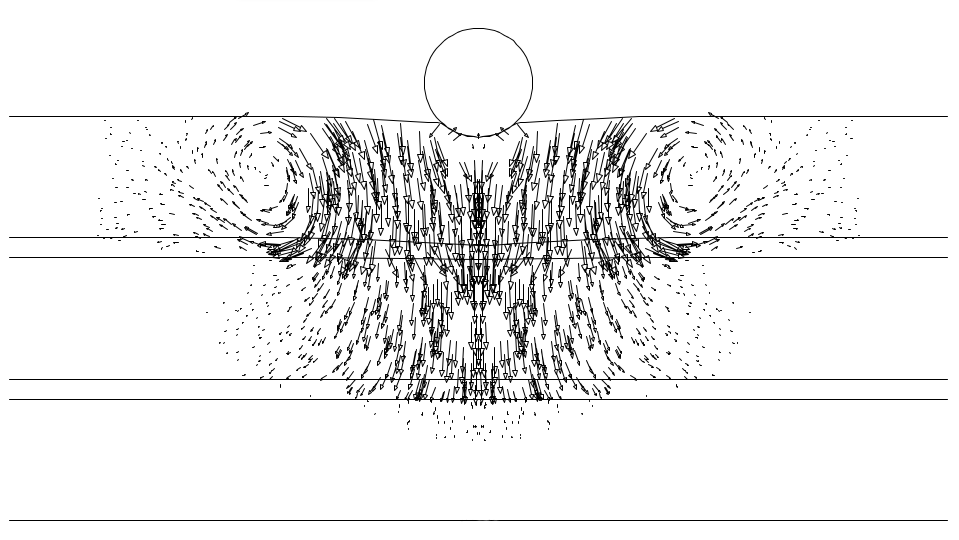
\includegraphics[width=\textwidth]{png/stounly-wave/01.png}
\caption{9 мкс}
\end{subfigure}
%\begin{subfigure}[b]{0.5\textwidth}
%\centering
%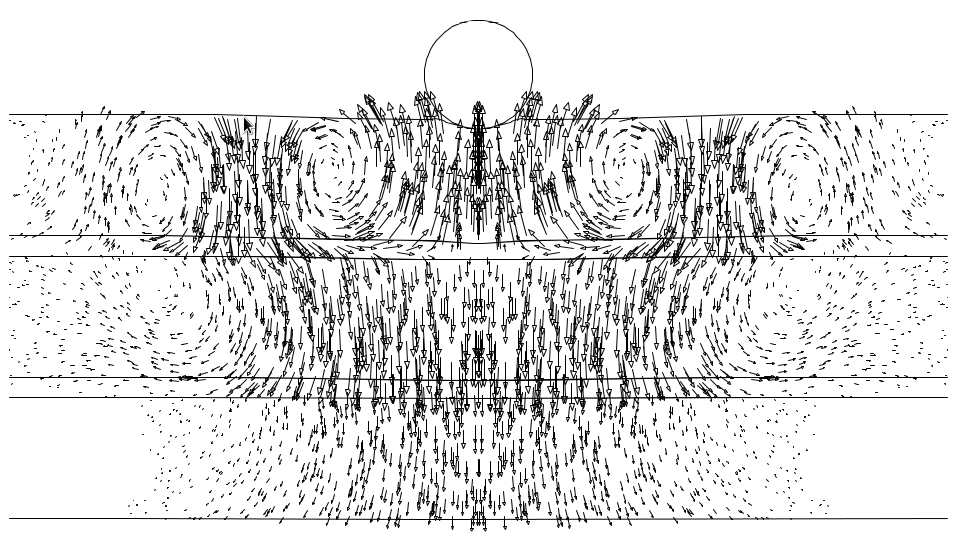
\includegraphics[width=\textwidth]{png/stounly-wave/02.png}
%\caption{15 мкс}
%\end{subfigure}
\begin{subfigure}[b]{0.5\textwidth}
\centering
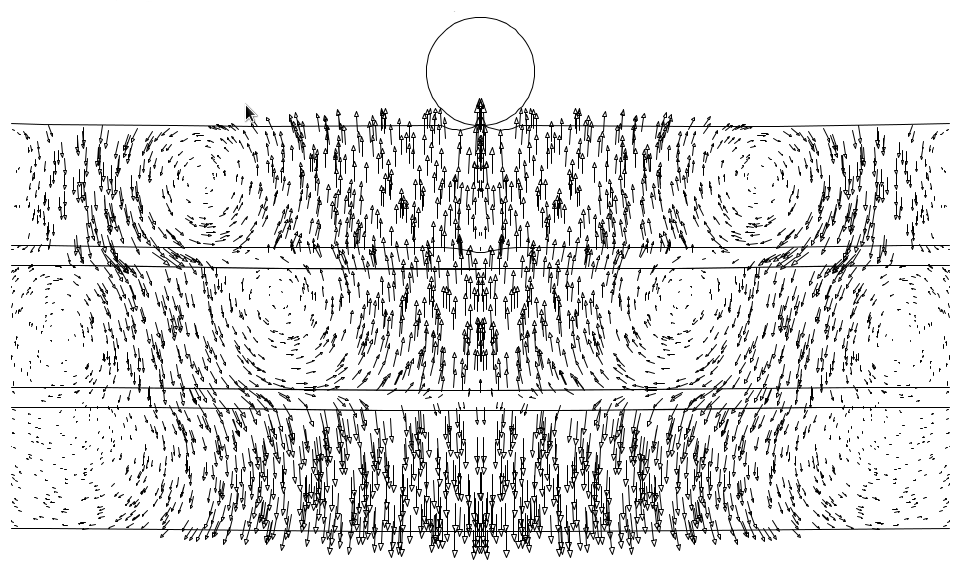
\includegraphics[width=\textwidth]{png/stounly-wave/03.png}
\caption{22.5 мкс}
\end{subfigure}
\caption{Формирование волн Стоунли в многослойной преграде.}
\label{pic:stounly_wave}
\end{figure}

Также в третьей главе обсуждается связь волновых процессов с различными критериями разрушения. В основных расчётах используются четыре критерия -- максимальное сжатие, максимальное растяжение, максимальное сдвиговое напряжение, энергия формоизменения (эквивалентное напряжение Мизеса). Данные критерии имеют ясный физический смысл, не требуют введения дополнительных констант и покрывают основные сценарии разрушения материала. Существуют сценарии, в которых данные критерии разрушения соотносятся с практикой неудовлетворительно, и требуется применение критериев Мора и Друкера-Прагера. Такие случаи необходимо рассматривать отдельно, в том числе определять необходимые константы для материалов.

Результаты модельного расчёта соударения ударника и монолитной преграды представлены на рис. \ref{pic:destruction_test}. Показаны максимальные значения напряжений в каждой точке за всё время соударения.

\begin{figure}[htp]
\centering
\begin{subfigure}[b]{0.45\textwidth}
\centering
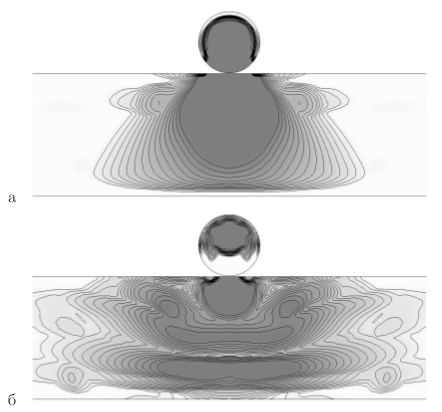
\includegraphics[width=\textwidth]{png/destruction_test-1.png}
\end{subfigure}
\begin{subfigure}[b]{0.45\textwidth}
\centering
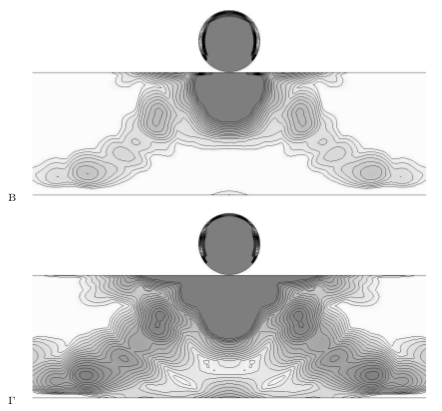
\includegraphics[width=\textwidth]{png/destruction_test-2.png}
\end{subfigure}
\caption{Тестирование критериев разрушения: а - сжимающие напряжения, б - растягивающие напряжения, в - сдвиговые напряжения, г – напряжение Мизеса.}
\label{pic:destruction_test}
\end{figure}

В завершение третьей главы рассматривается задача о вторичном ударе и взаимодействии упругой волны с зоной материала, разрушенного после первого импульса нагрузки. Рассматриваются сетки разной мелкости и их влияние на качество решения. Прохождение волны через зону разрушенного материала показано на рис. \ref{pic:crack_final_front}.

\begin{figure}[htp]
\begin{subfigure}[b]{0.5\textwidth}
\centering
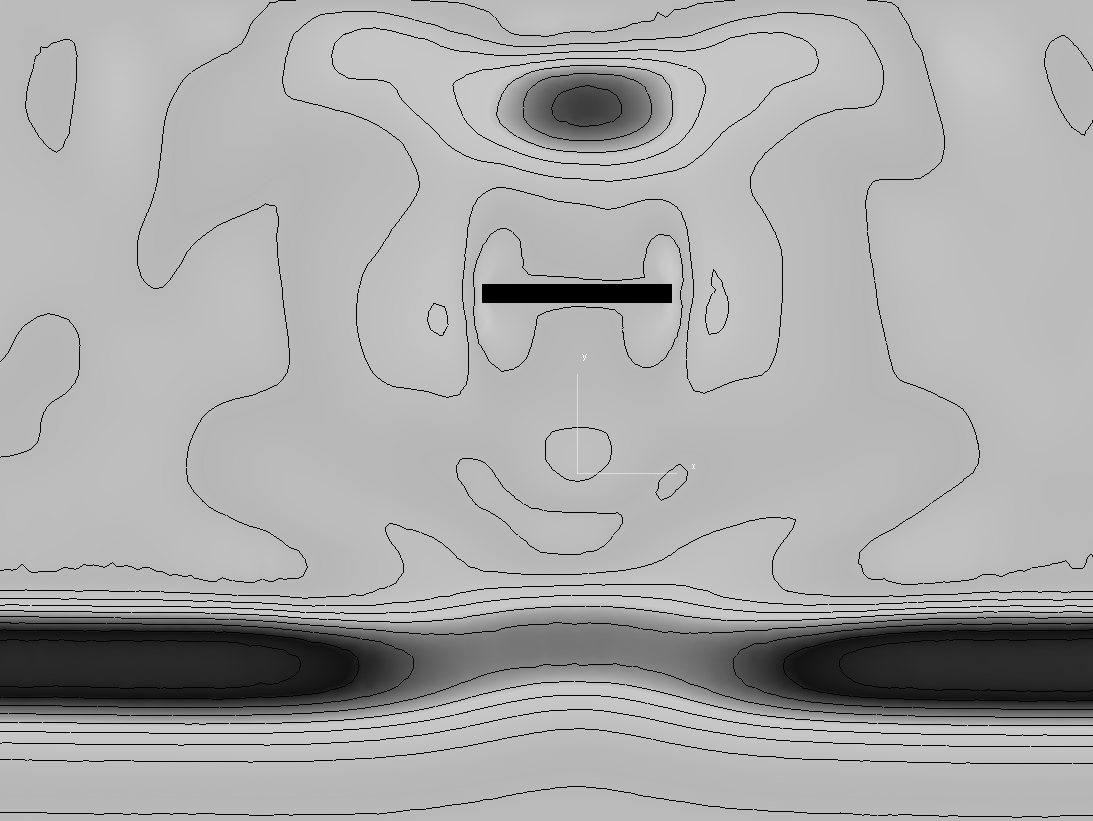
\includegraphics[width=\textwidth]{png/wave-around-crack/final-front-uniform-mesh.png}
\caption{Однородная мелкая сетка.}
\end{subfigure}
\begin{subfigure}[b]{0.5\textwidth}
\centering
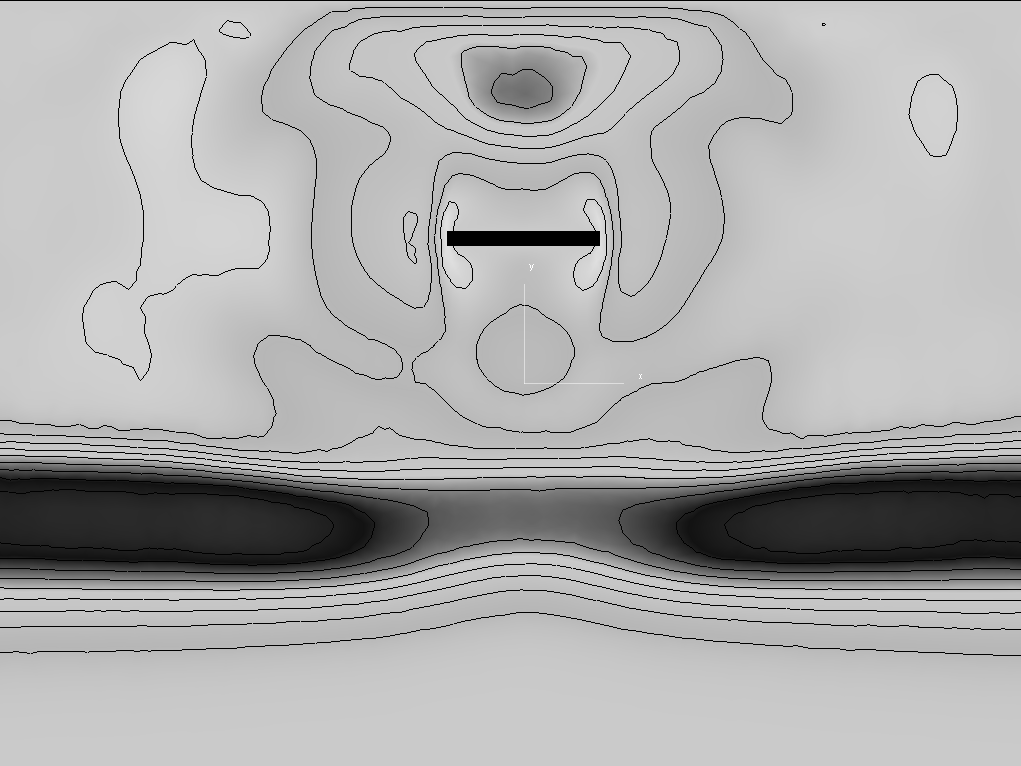
\includegraphics[width=\textwidth]{png/wave-around-crack/final-front-non-uniform-mesh.png}
\caption{Сетки разной мелкости.}
\end{subfigure}
\caption{Отражённая волна и восстановление фронта проходящей волны за раздробленной областью.}
\label{pic:crack_final_front}
\end{figure}

%\clearpage
%\newpage

\subsubsection*{Глава 4}

В четвертой главе решается задача о низкоскоростном динамическом нагружении элемента композитной обшивки и силового кессона крыла самолёта. На рис. \ref{pic:construction} приведена схема строения обшивки и силового кессона крыла. Обшивка толщиной 6.5~мм состоит из 3 композитных субпакетов, стрингер толщиной 13~мм -- из 6 аналогичных субпакетов. Каждый субпакет состоит из 11 монослоёв со взаимной ориентацией при укладке 45/0/-45/0/0/90/0/0/-45/0/45. Каждый монослой имеет следующий состав: 60\% -- ориентированные длинные углепластиковые волокна; 40\% -- матрица (эпоксидная смола). 

\begin{figure}[htp]
\center{\includegraphics[width=0.6\textwidth]{png/construction.png}}
\caption{Обшивка и силовой кессон крыла.}
\label{pic:construction}
\end{figure}

Проведены расчеты для двух постановок эксперимента -- удар по отдельному элементу обшивки и удар по элементу обшивки со стрингером (рис. \ref{pic:pkm_problem}). Для задачи со стрингером рассмотрены постановки с центральным и нецентральным ударом.

\begin{figure}[htp]
\centering
\begin{subfigure}[b]{0.45\textwidth}
\centering
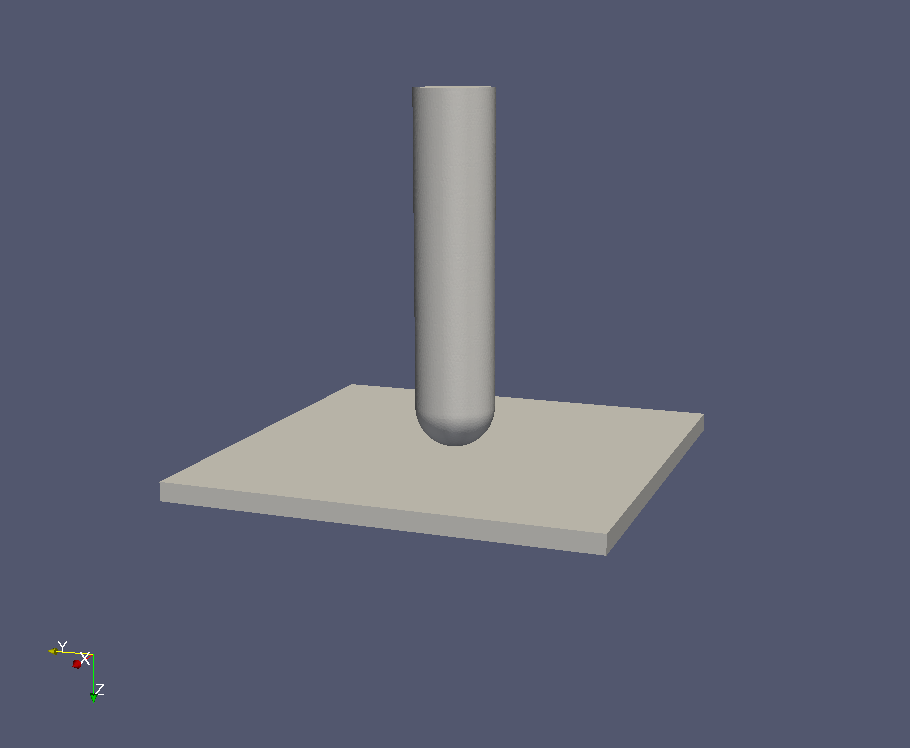
\includegraphics[width=\textwidth]{png/pkm-experiment/wing-only/scene.png}
\caption{Одиночный элемент обшивки.}
\end{subfigure}
\begin{subfigure}[b]{0.45\textwidth}
\centering
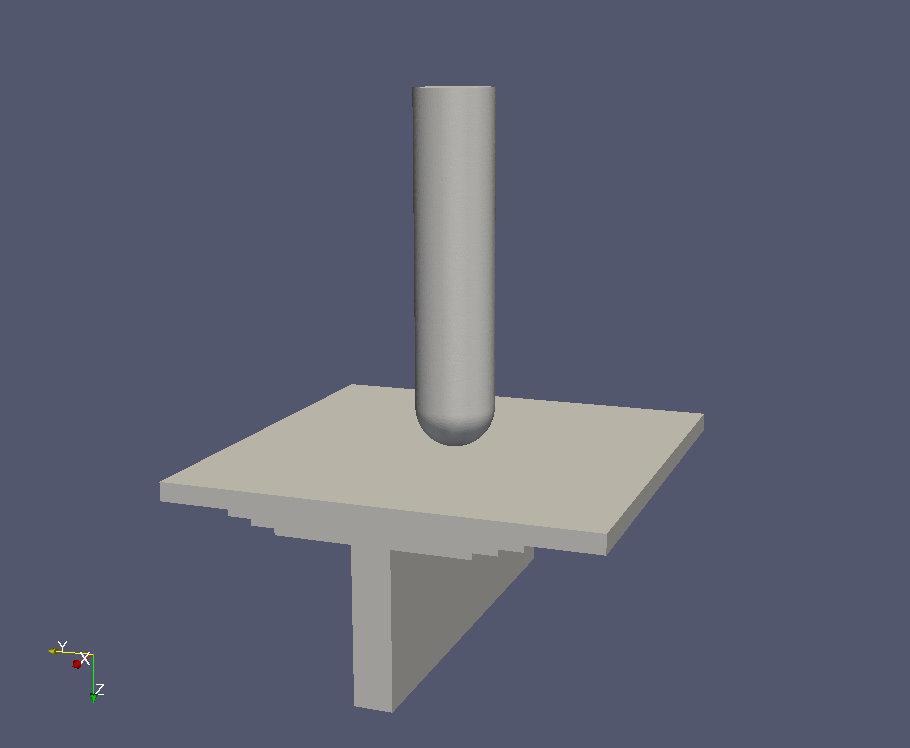
\includegraphics[width=\textwidth]{png/pkm-experiment/wing-stringer/scene.png}
\caption{Элемент обшивки со стрингером.}
\end{subfigure}
\caption{Вид расчётной области в задаче о низкоскоростном динамическом нагружении элемента композитной обшивки и силового кессона крыла самолёта.}
\label{pic:pkm_problem}
\end{figure}

Для всех постановок получены области концентрации напряжений, вызванные волновыми процессами в ходе соударения. Определены зоны потенциальных повреждений конструкции, обусловленные разными механизмами разрушения материала (рис. \ref{pic:pkm_experiment_compare_integral} и \ref{pic:pkm_experiment_compare_tension}). Для элемента обшивки без стрингера размер разрушенной области составляет 50-60 мм, для элемента обшивки со стрингером 25-30 мм при центральном ударе и 20-25 мм при нецентральном ударе. Получено, что наличие стрингера существенно разгружает элемент обшивки при динамическом воздействии и уменьшает размер потенциально повреждённых областей. Данный результат важен, так как при действии статической нагрузки наличие стрингера напротив вызывает концентрацию напряжений и приводит к разрушению при меньшей силе воздействия.

\begin{figure}[htp]
\centering
\begin{subfigure}[b]{0.3\textwidth}
\center
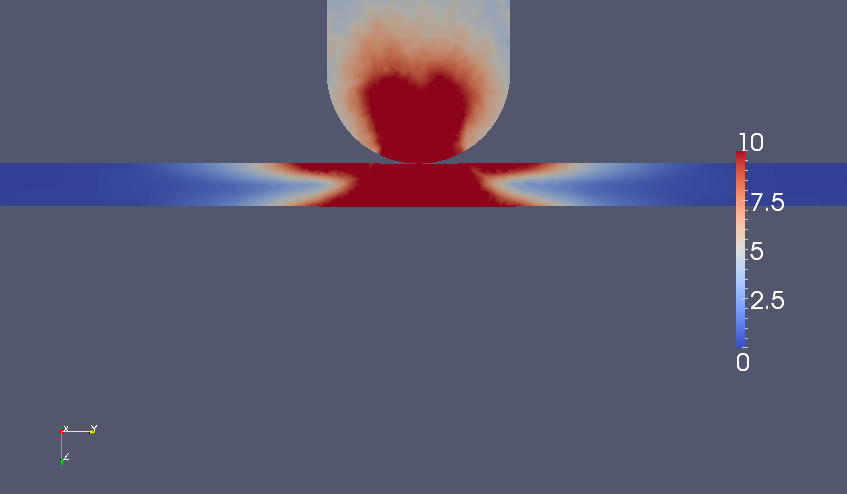
\includegraphics[width=\textwidth]{png/pkm-experiment/wing-only/sum.png}
\end{subfigure}
\begin{subfigure}[b]{0.3\textwidth}
\center
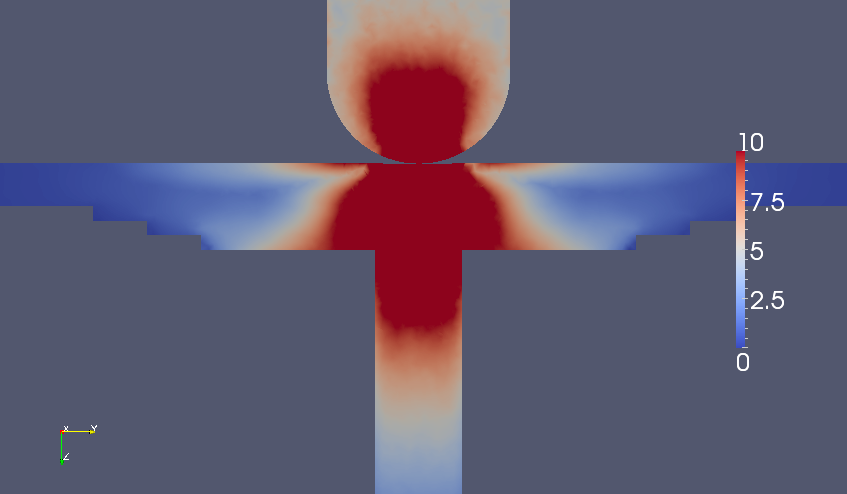
\includegraphics[width=\textwidth]{png/pkm-experiment/wing-stringer/sum.png}
\end{subfigure}
\begin{subfigure}[b]{0.3\textwidth}
\center
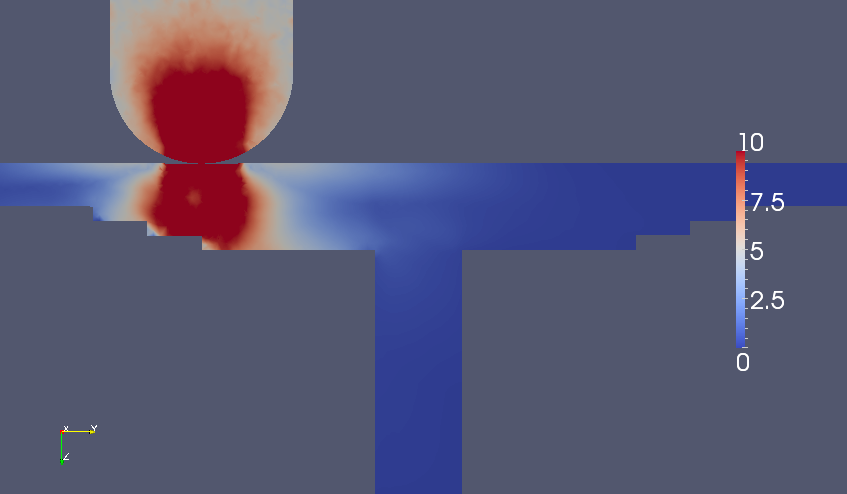
\includegraphics[width=\textwidth]{png/pkm-experiment/wing-stringer-non-center/sum.png}
\end{subfigure}
\caption{Потенциальные области разрушений по критерию интегрального воздействия.}
\label{pic:pkm_experiment_compare_integral}
\end{figure}

\begin{figure}[htp]
\centering
\begin{subfigure}[b]{0.3\textwidth}
\center
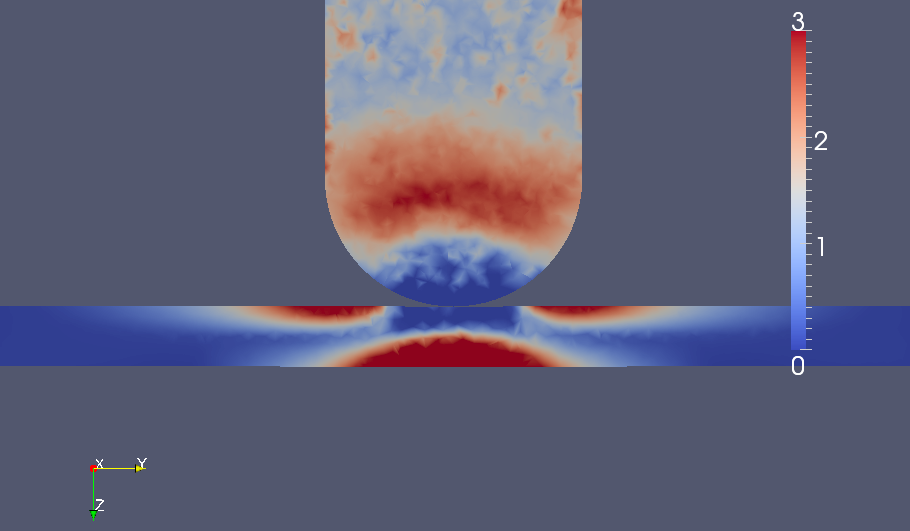
\includegraphics[width=\textwidth]{png/pkm-experiment/wing-only/tension-2.png}
\end{subfigure}
\begin{subfigure}[b]{0.3\textwidth}
\center
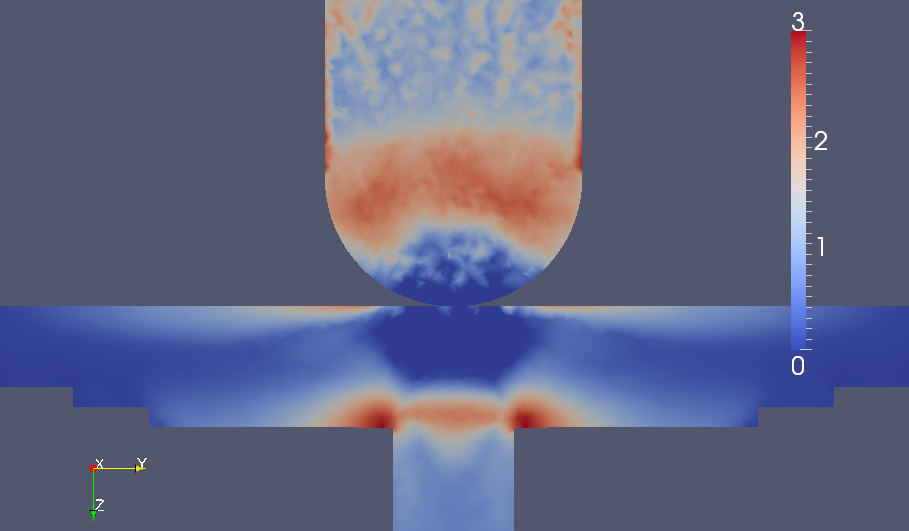
\includegraphics[width=\textwidth]{png/pkm-experiment/wing-stringer/tension-2.png}
\end{subfigure}
\begin{subfigure}[b]{0.3\textwidth}
\center
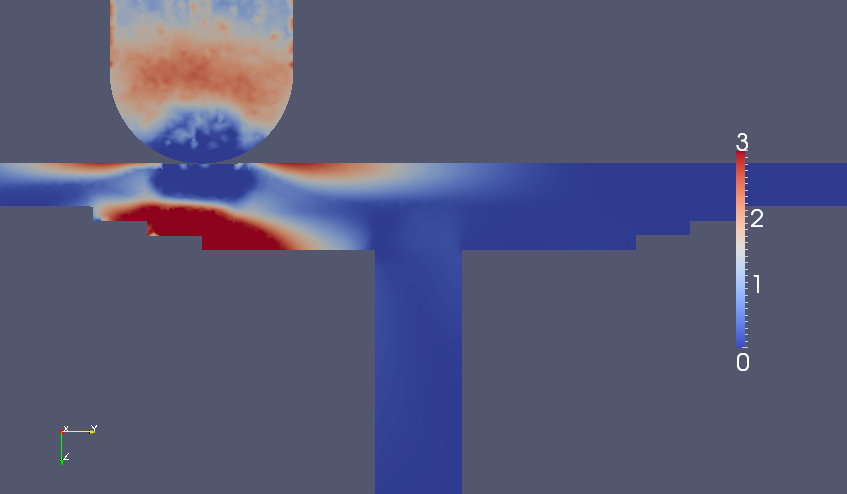
\includegraphics[width=\textwidth]{png/pkm-experiment/wing-stringer-non-center/tension-2.png}
\end{subfigure}
\caption{Потенциальные области разрушений по критерию растягивающих напряжений.}
\label{pic:pkm_experiment_compare_tension}
\end{figure}

Более подробное описание протекающих процессов приведено в тексте диссертации.

\clearpage
\newpage

\subsubsection*{Глава 5}

В пятой главе разработанные методы применяются для решения ряда задач биомеханики. Выполняется численное моделирование задач о черепно-мозговой травме, о динамическом нагружении согнутого коленного сустава, об ударе по торсу в защитной конструкции. Для всех задач получены картины распространения возмущения от удара и зоны концентрации напряжений, в которых возможны повреждения тканей и внутренних органов.

На рис. \ref{pic:knee_res_2} приведен один из результатов для задачи о коленном суставе -- распределение напряжений для постановки, в которой возможны как повреждения мениска, так и переломы. На рис. \ref{pic:chest_res} приведена картина распределения напряжений в задаче удара по торсу в защитной конструкции для момента максимальных напряжений в области сердечной мышцы. На рис. \ref{pic:cranium_2d_1d} показано распределение напряжений в многослойной конструкции покровов мозга при ударе. Более подробные результаты можно найти в тексте диссертации.

\begin{figure}[H]
\centering
\begin{subfigure}[b]{0.4\textwidth}
\centering
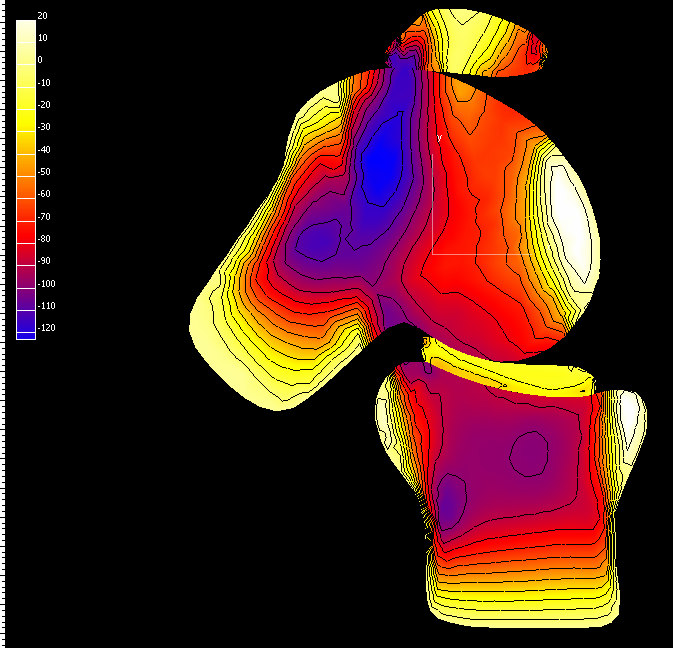
\includegraphics[width=\textwidth]{png/cranium/knee-res-2.png}
\caption{Начальный момент удара}
\end{subfigure}
\begin{subfigure}[b]{0.4\textwidth}
\centering
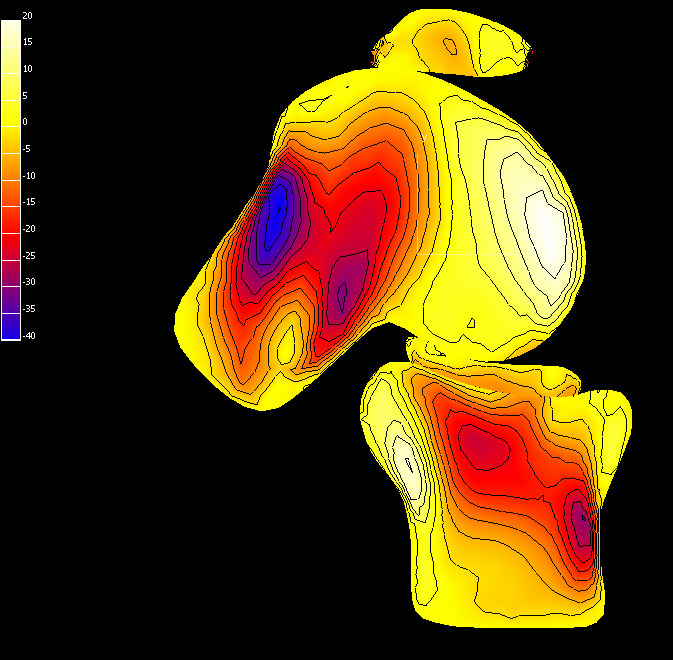
\includegraphics[width=\textwidth]{png/cranium/knee-res-3.png}
\caption{Завершающая стадия удара}
\end{subfigure}
\caption{Задача о нагружении коленного сустава. Распределение напряжений сжатия / растяжения. Скорость удара 9 м/с.}
\label{pic:knee_res_2}
\end{figure}

\begin{figure}[H]
\centering
\begin{subfigure}[b]{0.6\textwidth}
\centering
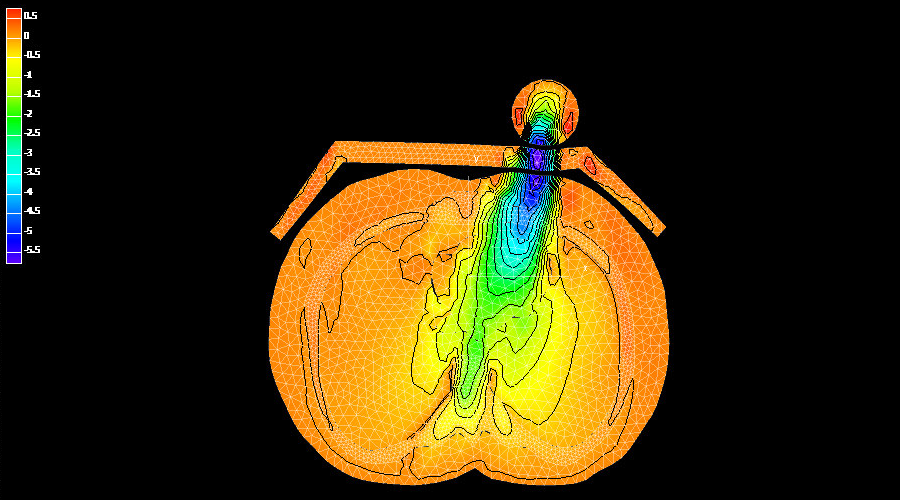
\includegraphics[width=\textwidth]{png/cranium/chest-res-06.png}
\end{subfigure}
%\begin{subfigure}[b]{0.9\textwidth}
%\centering
%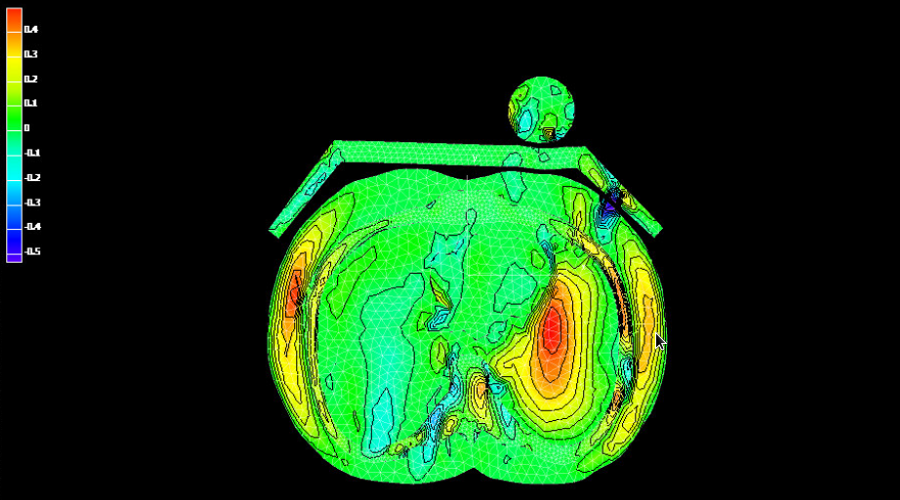
\includegraphics[width=\textwidth]{png/cranium/chest-res-07.png}
%\caption{Завершающая стадия соударения, отскок ударника}
%\end{subfigure}
\caption{Задача об ударе по торсу в защитной конструкции. Момент максимальной концентрации напряжений в области сердечной мышцы.}
\label{pic:chest_res}
\end{figure}

\begin{figure}[H]
\centering
\begin{subfigure}[b]{0.3\textwidth}
\centering
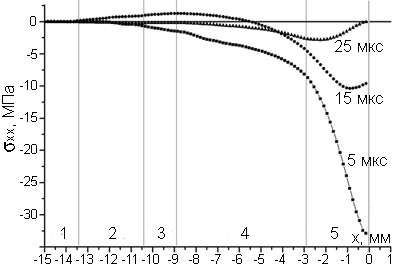
\includegraphics[width=\textwidth]{png/cranium/2d-sxx-1d.png}
\caption{$\sigma_{xx}$}
\end{subfigure}
\begin{subfigure}[b]{0.3\textwidth}
\centering
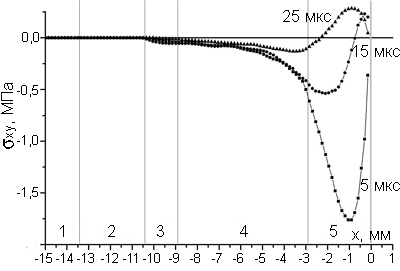
\includegraphics[width=\textwidth]{png/cranium/2d-sxy-1d.png}
\caption{$\sigma_{xy}$}
\end{subfigure}
\begin{subfigure}[b]{0.3\textwidth}
\centering
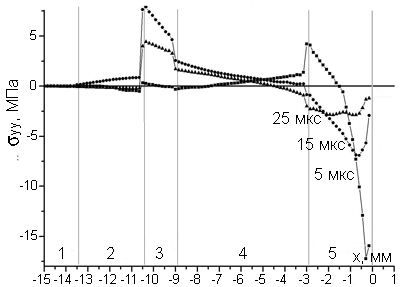
\includegraphics[width=\textwidth]{png/cranium/2d-syy-1d.png}
\caption{$\sigma_{yy}$}
\end{subfigure}
\caption{Задача о волновых процессах в покровах мозга. Зависимость напряжения от координаты. 1 -- мозговое вещество, 2 -- ликвор, 3 -- внутренний слой компактной костной ткани, 4 -- слой губчатой костной ткани, 5 -- внешний слой компактной костной ткани.}
\label{pic:cranium_2d_1d}
\end{figure}

Полученные результаты моделирования задач биомеханики показывают возможность применения разработанного метода для расчёта не только технических, но и биологических конструкций со сложной структурой и реологическими свойствами.

\subsubsection*{Заключение}

В заключении приводятся основные результаты и выводы, полученные в ходе выполнения работы.


\subsection*{Основные результаты и выводы диссертации}

\begin{enumerate}

\item Разработана математическая модель панели из полимерного композиционного материала для задачи о низкоскоростном ударе по элементу композитной конструкции. Модель может быть использована в том числе для более сложных инженерных конструкций, выполненных из композиционных материалов.

\item Разработан сеточно-характеристический метод численного моделирования задач механики деформируемого твердого тела на неструктурированной сетке в случае трех пространственных переменных. Основной особенностью метода является возможность выполнять расчёты с шагом $\tau > h / \lambda$.

\item Разработан алгоритм параллельной версии сеточно"=характеристического метода на неструктурированных сетках с явным выделением контактных границ для задачи многих тел. Реализован параллельный детектор столкновений для случая движения и деформации объектов.

\item Разработанный метод реализован в виде параллельного вычислительного комплекса. Выполнена интеграция программного комплекса с программами задания геометрии объектов (Gmsh, Tetgen, Ani3D) и визуализации результатов расчётов (Paraview, Mayavi).

\item Выполнено численное исследование волновых процессов в многослойных средах. Для задач об объёмных волнах, поверхностных волнах, волнах на контактной границе получены поля скоростей и напряжений.

\item Выполнен анализ причин внутреннего повреждения элемента композитной обшивки и силового кессона крыла самолета при низкоскоростном ударе. Получены области повреждения конструкции, вызванные волновыми процессами в ходе соударения.

\item Получено численное решение задач о черепно-мозговой травме, о динамическом нагружении коленного сустава и об ударе по торсу в защитной конструкции.

\end{enumerate}


\subsection*{Список публикаций соискателя по теме диссертации}

\begin{enumerate}
\item Агапов П.И., Васюков А.В., Петров И.Б. Компьютерное моделирование волновых процессов в покровах мозга при черепно-мозговой травме. // Сборник научных трудов <<Процессы и методы обработки информации>>. М.: МФТИ, 2006. С. 154--163.
\item Агапов П.И., Васюков А.В. Компьютерное моделирование биомеханических процессов в покровах мозга. // Труды 49-й научной конференции МФТИ <<Современные проблемы фундаментальных и прикладных наук>>: Часть VII. Управление и прикладная математика. М.: <<Солар>>, 2007. С. 41--42.
\item Васюков А.В., Петров И.Б. Компьютерное моделирование биомеханических процессов в покровах мозга при динамическом нагружении. Сравнение механических моделей. // Сборник научных трудов <<Моделирование процессов обработки информации>>. М.: МФТИ, 2007. С. 67--76.
\item Васюков А.В., Петров И.Б. О разработке параллельной версии сеточно-характеристического метода для трехмерных уравнений механики деформируемого твердого тела. // Сборник научных трудов <<Модели и методы обработки информации>>. М.: МФТИ, 2009. С. 13--17.
\item Васюков А.В., Петров И.Б., Стрижевская А.Д. Компьютерное моделирование волновых процессов в гидроупругих средах сеточно"=характеристическим методом. // Сборник научных трудов <<Модели и методы обработки информации>>. М.: МФТИ, 2009. С. 18--22.
\item Васюков А.В., Петров И.Б., Черников Д.В. О сеточно-характеристическом численном методе на неструктурированных сетках для задач механики деформируемого твердого тела в случае трех пространственных переменных. // Сборник научных трудов <<Информационные технологии: модели и методы>>. М.: МФТИ, 2010. С. 52--57.
\item Болоцких Ю.В., Васюков А.В., Петров И.Б. О численном решении некоторых задач биомеханики. // Сборник научных трудов <<Информационные технологии: модели и методы>>. М.: МФТИ, 2010. С. 58--64.
\item Васюков А.В., Петров И.Б. Моделирование механических факторов черепно"=мозговых травм сеточно"=характеристическим численным методом. // Вестник Российского государственного университета им. И.Канта. Калининград: БФУ им. И.Канта, 2010, вып.10. С. 42--51.
\item Васюков А.В., Петров И.Б. Компьютерное моделирование последствий механических черепно"=мозговых травм. // Информационные технологии, 2011, №5. С. 58--62.
\item I. Petrov, Y. Bolotskikh and A. Vasyukov. Modeling of Dynamic Problems in Biomechanics. // Math. Model. Nat. Phenom. 2011, Vol. 6, No. 7, pp. 70--81.
\item Igor Petrov, Alexey Vasyukov, Dmitry Chernikov, Yulia Bolotskikh. Modeling of dynamic problems in biomechanics using HPC clusters. // The 8th Congress of the International Society for Analysis, its Applications, and Computation. Book of Abstracts. -- M.: PFUR, 2011 -- P. 342.
\item Васюков А.В. О решении задач динамической прочности трубопроводов под давлением с использованием параллельной версии сеточно"=характеристического численного метода на неструктурированных сетках. // Труды 54-й научной конференции МФТИ <<Проблемы фундаментальных и прикладных естественных и технических наук в современном информационном обществе>>. Том 2. Управление и прикладная математика. М.: МФТИ, 2011. С. 60--61.
% ISAAC 2011 - статья
% ФУПМ 2012
\end{enumerate}

\subsection*{Личный вклад соискателя в работах с соавторами}

В части моделей соискателем разработана математическая модель панели из полимерного композиционного материала для задачи о низкоскоростном ударе по элементу композитной обшивки и силового кессона крыла самолёта. Также выполнено исследование свойств матрицы общего вида $A_q$, возникающей при программной реализации модели.

В части численных методов соискателем предложен и реализован сеточно-характеристический метод, позволяющий выполнять расчёты с шагом $\tau > h / \lambda$ в трёхмерной постановке. Выполнено исследование разработанного метода на аппроксимацию и устойчивость. Проведено тестирование реализации метода.

В части программной реализации метода и разработки параллельного вычислительного комплекса соискателем разработан и реализован алгоритм параллельной версии численного метода, предложен алгоритм параллельного детектора столкновений, выполнена интеграция программного комплекса с программами задания геометрии объектов (Gmsh, Tetgen, Ani3D) и визуализации результатов расчётов (Paraview, Mayavi).

В части проведения расчетов и анализа результатов соискателем выполнено численное исследование волновых процессов в многослойных средах, моделирующих панель из полимерного композиционного материала при динамическом нагружении, получены области потенциальных разрушений различных типов, обусловленных распространением и взаимодействием волновых фронтов в материале. Проведено численное моделирование натурного эксперимента по динамическому нагружению элемента композитной обшивки и силового кессона крыла самолёта для двух постановок эксперимента -- удар по отдельному элементу обшивки и удар по элементу обшивки со стрингером. Для задачи со стрингером рассмотрены постановки с центральным и нецентральным ударом. Выполнен анализ областей концентрации напряжений, вызванных волновыми процессами в ходе соударения. Определены зоны потенциальных повреждений конструкции, обусловленные разными механизмами разрушения материала.

Проведено численное исследование волновых процессов в покровах мозга при динамическом нагружении для многокомпонентной и упрощенных моделей. Выполнены расчеты задач о черепно-мозговой травме, о нагружении коленного сустава, об ударе по торсу в защитной конструкции.

